\documentclass{standalone}

\usepackage{tikz}
\usepackage{pgfplots}
\usepgfplotslibrary{statistics}
\usetikzlibrary{pgfplots.statistics}
\usepackage{etoolbox}
\pgfplotsset{compat=1.12}

\newtoggle{label}
\togglefalse{label}

\begin{document}
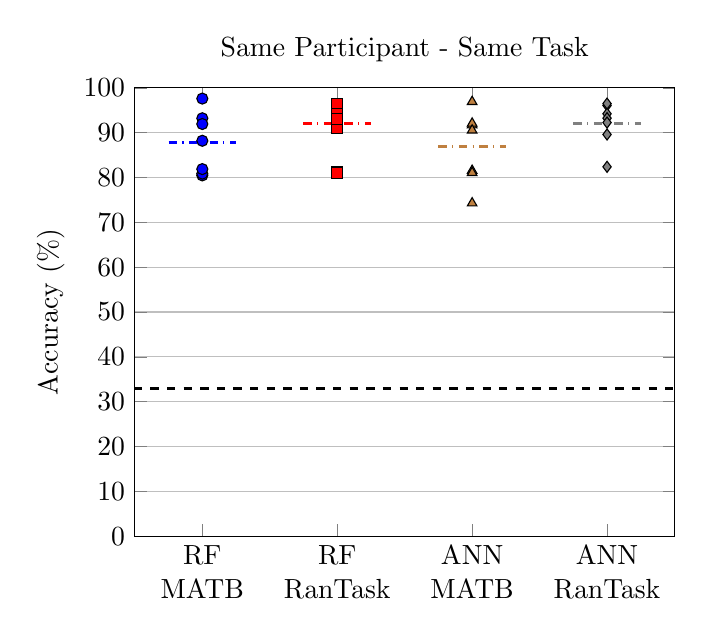
\begin{tikzpicture}
\begin{axis}[
	ymajorgrids,
	scatter/classes= {
		a={mark=*, fill=blue, draw=black, mark size=2},
		b={mark=square*, fill=red, draw=black},
		c={mark=triangle*, fill=brown, draw=black},
		d={mark=diamond*, fill=gray, draw=black}
	},
	ymin=0,
	ymax=100,
	xmin = .5, 
	xmax=4.5,
	ytick={0,10,...,100},
	xtick={1,2,3,4},
	xticklabel style={align=center},
	xticklabels={RF\\MATB, RF\\RanTask, ANN\\MATB, ANN\\RanTask},
	title=Same Participant - Same Task, 
	ylabel=Accuracy (\%)]

	\addplot+[ mark=None, dashed, black, line width = 1pt ]
	coordinates {
	(0, 33)
	(5, 33)	
};

	% Random Forest MATB
	\addplot+[ scatter,
			only marks,
			scatter src=explicit symbolic]
	coordinates {
			(1, 80.48) [a]
			(1, 97.61) [a]
			(1, 80.87) [a]
			(1, 88.20) [a]
			(1, 93.22) [a]
			(1, 91.94) [a]
			(1, 81.88) [a]
};

	% Random Forest MATB Mean
	\addplot+[ mark=None, dashdotted, blue, line width = 1pt ] 
	coordinates {
		(0.75, 87.74)
		(1.25, 87.74)
};

	% Random Forest RanTask
	\addplot+[ only marks,
			scatter,
			scatter src=explicit symbolic]
	coordinates {
			(2, 81.11)	[b]
			(2, 94.94)	[b]
			(2, 90.99)	[b]
			(2, 93.83)	[b]
			(2, 96.43)	[b]
			(2, 94.09)	[b]
			(2, 92.97)	[b]
};

	% Random Forest RanTask Mean
	\addplot+[ mark=None, dashdotted, red, line width = 1pt ] 
	coordinates {
		(1.75, 92.05)
		(2.25, 92.05)
};

	% ANN MATB
	\addplot+[ only marks,
			scatter,
			scatter src=explicit symbolic]
	coordinates {
			(3, 74.29)	[c]
			(3, 96.91)	[c]
			(3, 81.55)	[c]
			(3, 91.71)	[c]
			(3, 92.08)	[c]
			(3, 90.54)	[c]
			(3, 81.07)	[c]
};

	% ANN MATB Mean
	\addplot+[ mark=None, dashdotted, brown, line width = 1pt ] 
	coordinates {
		(2.75, 86.87)
		(3.25, 86.87)
};

	% ANN RanTask
	\addplot+[ only marks,
			scatter,
			scatter src=explicit symbolic]
	coordinates {
			(4, 82.39)	[d]
			(4, 96.07)	[d]
			(4, 89.60)	[d]
			(4, 96.49)	[d]
			(4, 94.22)	[d]
			(4, 93.24)	[d]
			(4, 92.26)	[d]
};

	% ANN RanTask Mean
	\addplot+[ mark=None, dashdotted, gray, line width = 1pt ] 
	coordinates {
		(3.75, 92.03)
		(4.25, 92.03)
};

\end{axis}
\end{tikzpicture}

\end{document}
















